%\linenumbers*
\chapter{EFFECT OF CONTINUOUS AND DISCONTINUOUS STORM}
\label{sec:EFFECTSOFCONTINOUSANDDISCONTINUSSTORM}

\section{Introduction}
\label{sec:ContinousAndDiscontinousStormIntroduction}
This chapter investigates the effect of no-rain periods within a storm
that is termed as WSP (Within-Storm Pause) on soil erosion estimations.
Continuous and discontinuous storms are distinguished by the existence of WSPs
within the storm duration.

% In this chapter, no-rain periods within a storm is termed as WSP
% (Within-Storm Pause).

\section{Simulation Data and Methods}
\label{sec:ContinousAndDiscontinousStormMethods}

Three process-based models---WEPP, EUROSEM and RillGrow---were used for
runoff and soil loss simulations. Three erosion models were used to highlight
the effect of WSP on erosion estimations. Although the outputs from three
erosion models could give three very different results---this actually was the
case, employing all three models will give a stronger argument that the removal
of WSPs does (or does not) have an impact on runoff and soil loss simulations.
The main aim of this investigation is to find out whether WSPs influence runoff
and soil loss generations. The more important question is, however, how WSPs
influence runoff and soil erosion. This is more difficult to answer even when a
single erosion model was used.

Event rainfall recorded on 11 October 2000 in Southover (Table
\ref{tab:DetailsOfDataStations}) was subjectively selected. This event includes
a number of WSPs in the total storm duration. The total rainfall amount is 89.9
mm. This event was considered to be responsible for the severe flood incidents
in the study region \citep{boardman2001-346}.

As CLIGEN data removes WSPs by its design specification, only breakpoint data
type, which retains WSPs, was used in this chapter. Breakpoint event rainfall
data with 15-min timestep were used. The reason for the selection of 15-min time
scale have been discussed in Chapter
\ref{sec:EFFECTSOFTEMPORALSCALESOFSTROMDATA}. Hyetographs of the original
October event and the modified October event after removing WSPs are shown in
Figure \ref{fig:rainfall_discont_cont}. The rainfall intensities for each 15-min
interval are unchanged (Figure \ref{fig:rainfall_discont_cont}). WEPP and
EUROSEM were used to simulate runoff and soil loss using these data. Total
duration of the data with WSPs was 1230 minutes and 885 minutes without WSPs.

\begin{figure}[htpb]
  \centering
    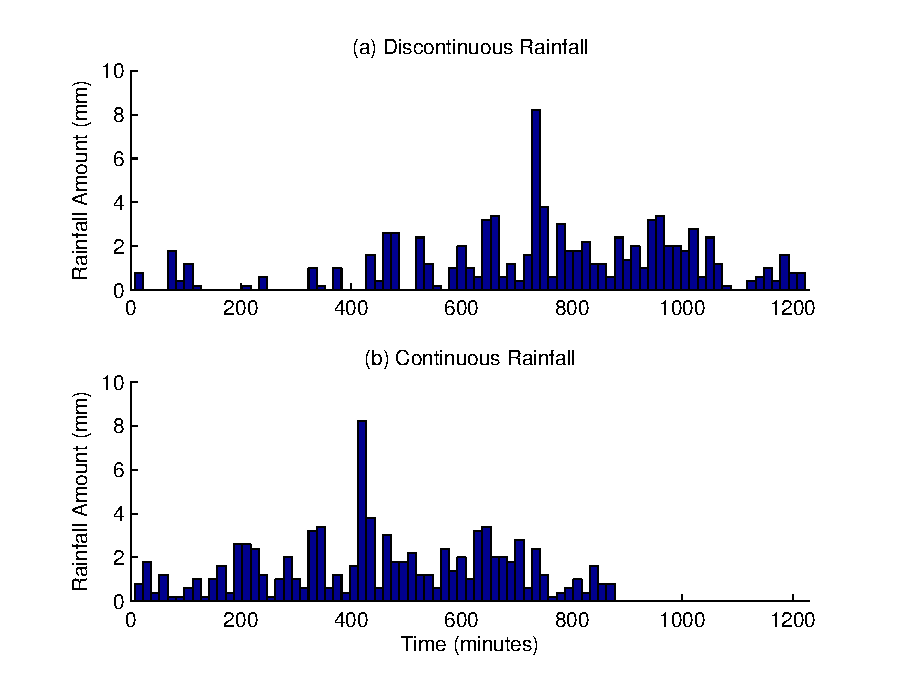
\includegraphics[width=0.8\textwidth]
{./img/rainfall_discont_cont_input}
  \caption[15-min rainfall data used for the investigations of effects of
continuous and discontinuous rainfall on soil erosion.]{15-min rainfall data
used for the investigations of effects of continuous and discontinuous rainfall
on soil erosion. (a) original 11 October 2000 event ;(b) modified 11 October
2000 event after removing WSPs}
  \label{fig:rainfall_discont_cont}
\end{figure}

Another set of continuous and discontinuous rainfall data were prepared for
RillGrow runs. As RillGrow simulates runoff and soil loss in great detail
temporally and spatially, rainfall with a relatively short duration and a pulse
of constant high intensity peaks were intentionally prepared (Figure
\ref{fig:rg2_input_continuous}).

\begin{figure}[htpb]
  \centering
    \subfloat[Continuous]{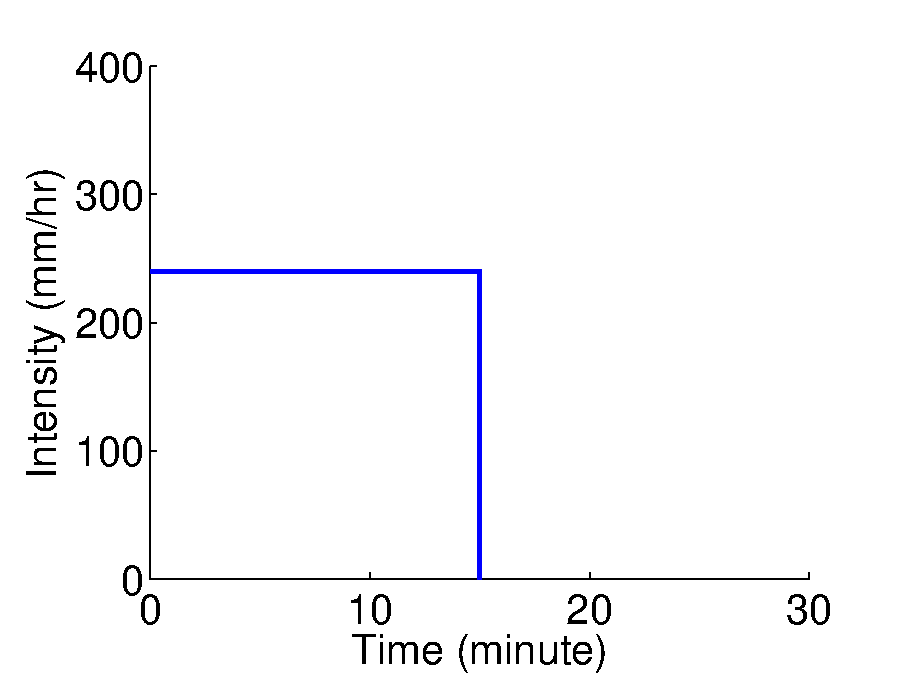
\includegraphics[width=0.45\textwidth]
{./img/rg2_input_continuous}}
    \subfloat[Discontinuous]{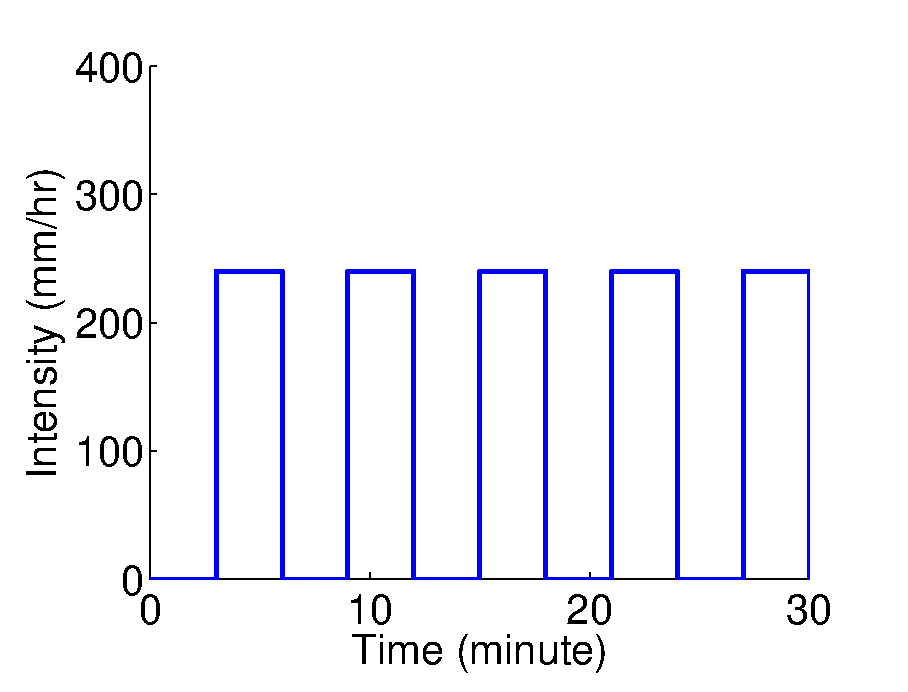
\includegraphics[width=0.45\textwidth]
{./img/rg2_input_discontinuous}}
  \caption{Continuous and Discontinuous rainfall for RillGrow simulations. Both
storms have the same total rainfall amount of 65.5 mm. Rainfall durations for
continuous (a) and discontinuous (b) rainfall are 15 minutes and 30 minutes,
respectively.}
  \label{fig:rg2_input_continuous}
\end{figure}

Runoff and soil loss rates were simulated with WEPP, EUROSEM and RillGrow using
the prepared rainfall data.

\section{Simulation Results}
\label{sec:InterStormGapsSimulatedResults}

%\subsection{WEPP}
%\label{sec:WEPPInterStormGapsRunoff}
WEPP estimated runoff amounts for continuous and discontinuous rainfall are
shown in Table \ref{tab:EstimatedRunoffForEachHillslope}. With continuous
rainfall, WEPP generated more runoff than with discontinuous rainfall. However,
WEPP estimated less soil loss with continuous rainfall than with discontinuous
rainfall. The soil loss rate increases 4.6 percent with a discontinuous storm in
comparison to the soil loss rate which is estimated by WEPP with a continuous
storm.

\begin{table}[hbtp]
  \figureversion{tabular}
  \centering
  \caption{WEPP estimated runoff and soil loss with continuous and discontinuous
rainfall for each hillslope}
  \label{tab:EstimatedRunoffForEachHillslope}
    \begin{tabular}{lll}
      \toprule
      & Runoff (mm)& Soil loss (t/ha) \\
      \midrule
      Continuous & 38.1 & 47.4 \\
      Discontinuous & 34.3 ($-$10.0) & 49.6 ($+$4.6)\\
      \bottomrule
      \multicolumn{3}{l}{\footnotesize Figures in (\ ) are the \% changes from
the result with a continuous storm.}
    \end{tabular}
\end{table}

EUROSEM estimated runoff and soil loss rates for continuous and discontinuous
rainfall are shown in Table
\ref{tab:EUROSEMEstimatedSoilLossRatesForEachHillslope}. With continuous
rainfall, EUROSEM generated more runoff than with discontinuous rainfall.
Also, EUROSEM estimated more soil loss with continuous rainfall than with
discontinuous rainfall. The runoff and soil loss rate decreases 11.9 and 12.7
percent, respectively, with a discontinuous storm in comparison to the soil loss
rate with a continuous storm.

\begin{table}[hbtp]
  \figureversion{tabular}
  \centering
  \caption{EUROSEM estimated runoff and soil loss with continuous and
discontinuous rainfall for each hillslope}
  \label{tab:EUROSEMEstimatedSoilLossRatesForEachHillslope}
    \begin{tabular}{lll}
      \toprule
                & Runoff (mm) & Soil loss (t/ha) \\
      \midrule
      Continuous & 28.7 & 11.0 \\
      Discontinuous & 25.3 ($-$11.9)& 9.6 ($-$12.7)\\
      \bottomrule
%     \addlinespace[1mm]
      \multicolumn{3}{l}{\footnotesize Figures in (\ ) are the \% changes from
the result with a continuous storm.}
    \end{tabular}
\end{table}

RillGrow estimated soil loss rates for continuous and discontinuous rainfall are
shown in Table
\ref{tab:RillGrowRunoffAndSoilLossWithContAndDiscontRainfall}. RillGrow
generated less runoff with continuous rainfall than with discontinuous rainfall.
With discontinuous rainfall, runoff actually increased 0.2 percent. However,
RillGrow estimated more soil loss with continuous rainfall than with
discontinuous rainfall. The soil loss rate decreases 1 percent with a
discontinuous storm in comparison to the soil loss rate with a continuous storm.
Magnitudes of changes for runoff and soil loss are very small compared to WEPP
and EUROSEM results.

\begin{table}[htbp]
  \figureversion{tabular}
  \centering
  \caption{RillGrow simulated runoff and soil loss with continuous and
discontinuous rainfall}
  \label{tab:RillGrowRunoffAndSoilLossWithContAndDiscontRainfall}
    \begin{tabular}{lll}
      \toprule
  & Totals lost from edges$^\dagger$ (litre) & Soil loss (t/ha) \\
      \midrule
      Continuous & 471.5 & 91.2 \\
      Discontinuous & 472.4 ($+$0.2)& 90.3 ($-$1.0)\\
      \bottomrule
%     \addlinespace[1mm]
      \multicolumn{3}{p{11cm}}{\footnotesize $^\dagger$ No infiltration was
considered. Every rain runs off the edge of the simulated plot. Figures in (\ )
are the \% changes from the result with a continuous storm.}
    \end{tabular}
\end{table}


\section{Discussion}
\label{sec:InterStormPeriodsWithinAStormDiscussion}

This investigation clearly shows the effect of removing WSPs during data
preparations for erosion simulations. By removing WSPs, we are unintentionally
creating a rainfall event with higher average intensity than original average
intensity as total storm duration becomes shortened. This decreased duration
means that the time given for the erosion simulation effectively decreases,
resulting in smaller time values for other relevant process calculations. This
may have effects on, for example, gross infiltration amounts and runoff
initiation times. This alteration clearly has effects on modelling
runoff and soil loss in general. In principle, removing WSPs during a storm will
result in overestimated erosion rates as well as overestimated runoff. This was
the case for EUROSEM simulations.

Simulation results from RillGrow runs showed very small differences between
continuous and discontinuous rainfall. The differences were almost negligible.
This could be caused by internal random number generator which is used for
generating raindrop size. Thus, the result may imply that RillGrow is not
sensitive to WSPs.

%This may be because of the proportion and total
%duration of no-rain periods in the storm. The magnitude of the effect and
%importance of no-rain periods may be dependent on the proportion of no-rain
%periods and the amount of rainfall.

%This investigation again does not have observed runoff and soil loss for
%the event. There are no lab experiments on effects of the gaps either.
%RillGrow could give a good comparative result.

%Does RillGrow agrees with Tony's work?
%Then this can be used only for pattern comparison (increased with increased
%and decreased with decreased?) This is not the real observation.

Using breakpoint data for erosion simulation will prevent the loss of WSP
information. Therefore, using CLIGEN data is not recommended for studies
like current research which investigates effects of rainfall intensity
changes on soil erosion. However, using breakpoint data for continuous long-term
simulation is realistically very difficult since preparing such input for
erosion modelling is a very labour intensive and tedious task.

WEPP estimated more soil loss for discontinuous rainfall than continuous
rainfall. This was unexpected. In theory, rainfall with a higher average
rainfall intensity with the same amount, hence shorter duration is expected to
produce more soil loss than rainfall with a low average intensity. However, the
opposite results were observed. This is because WEPP changed the intensity of
the original breakpoint data used for the simulation. When time intervals
shorter than an hour were used, WEPP reconstructs breakpoint data from the
original breakpoint data to ``WEPP-interpreted'' breakpoint data, which have
different intensity information from original data. Accumulated rainfall amount
and the number of breakpoints are the same, but because the time increments are
changed by WEPP, rainfall intensity of the original breakpoint data has been
changed. WEPP increased intensity peaks of discontinuous rainfall while it
decreased intensity peaks of continuous rainfall (Figure
\ref{fig:intensity_discontinuous_and_continuous}).

\begin{figure}[htbp]
  \centering
    \subfloat[Discontinuous]{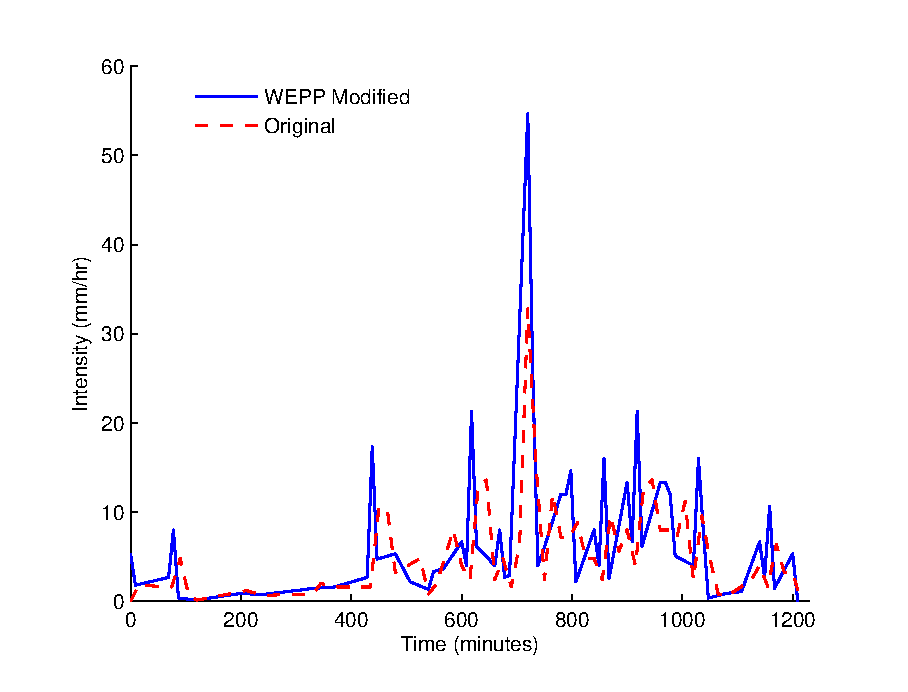
\includegraphics[width=0.45\textwidth]
{./img/intensity_discontinuous} \label{fig:intensity_discontinuous}}
    \subfloat[Continuous]{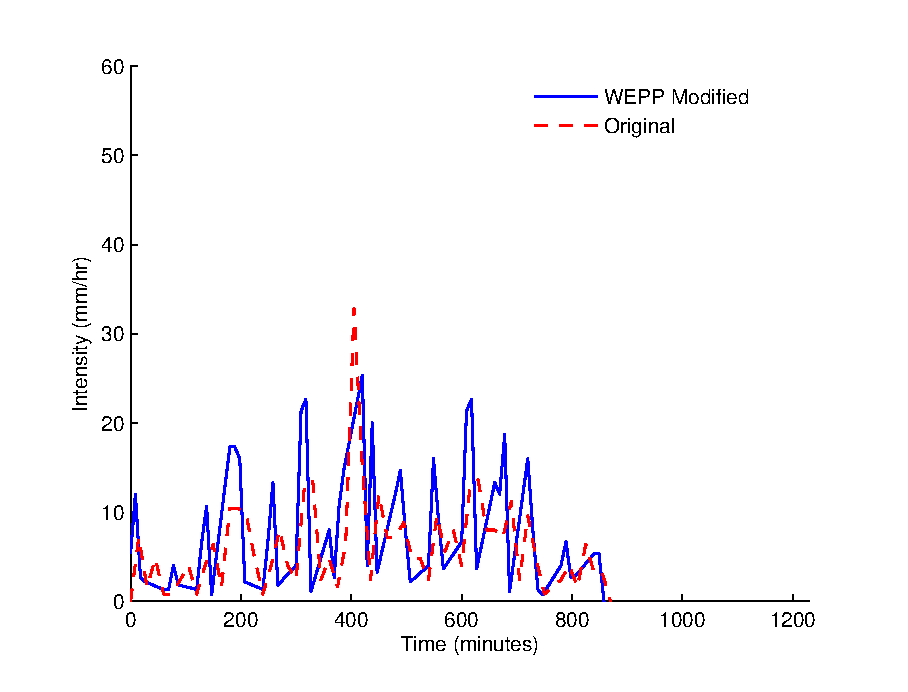
\includegraphics[width=0.45\textwidth]
{./img/intensity_continuous} \label{fig:intensity_continuous}}
  \caption{Original rainfall intensity and WEPP-modified rainfall intensity for
discontinuous and continuous rainfall.}
  \label{fig:intensity_discontinuous_and_continuous}
\end{figure}

WEPP elongates the peak intensity of discontinuous rainfall from 32.8 mm/hr to
54.7 mm/hr (Figure \ref{fig:intensity_discontinuous_and_continuous}). This is
about a 66.8\% increase in peak intensity. Since the rainfall amount and total
duration of discontinuous rainfall were kept almost the same, the average
rainfall intensity for the original (4.4 mm/hr) and WEPP modified (4.5 mm/hr)
rainfall were also similar.

This explains why WEPP estimated more soil losses for discontinuous rainfall.

%WEPP disaggregates the original rainfall into 10 breakpoints. When the
%rainfall lasts shorter than 60 min the number of breakpoints is reduced
%down to just one breakpoint even though the rainfall data have several
%breakpoints with a scale of 1-min, for example. When the rainfall duration
%is longer than 60-min, WEPP disaggregates the rainfall, even if the data
%scale is 1-min, into 10 breakpoints.
%
%Due to this behaviour of WEPP, the resulting runoff and soil loss may be
%estimated with large errors, considering the fact that rainfall intensity
%is different from the observation.
%
%Studies on impacts of rainfall intensity change on soil erosion with
%rainfall data shorter than hourly may result in runoff and soil loss
%estimations (by WEPP) which are different from the original.
%


\section{Conclusion}
\label{sec:InterStormPeriodsWithinAStormConclusion}

WSPs (Within-Storm Pauses) affected runoff and soil erosion simulations by WEPP
and EUROSEM. However, RillGrow showed almost no changes in runoff and soil
erosion simulations. Although it was not evident to conclude whether WSPs have
positive or negative effects on runoff and soil erosion estimations, removing
WSPs from rainfall data is not recommended for a study like this research.

%EUROSEM
%simulated decreased runoff and soil loss rates with rainfall data with WSPs.

Analyses of outputs from WEPP simulations revealed new problem. WEPP modifies
original rainfall intensity data and simulates erroneous results. When
breakpoint data with time scales shorter than 60-min temporal scale is used
for WEPP simulations, WEPP will re-construct the rainfall data so that original
rainfall intensity information is lost. Particularly, peak rainfall intensity
will be altered and shapes of rainfall storm will be changed. This clearly is a
major problem for current research as well as a major model fault for WEPP.
This means that, even if 15-min breakpoint rainfall data, as suggested
in the previous chapter, are used for WEPP simulations, rainfall data that WEPP
actually uses for the simulation will have different rainfall intensity.

%\nolinenumbers

%but how much different? no can say about real world, but certainly
%important when models are used. this means it is important to know how much
%``gaps'' in the storm in order to predict future soil erosion, particularly
%in relation to rainfall intensity changes.
%
%We learn that it is a best practice to use rainfall data which have all
%necessary information for modelling.

%What is the effect of the ``gaps''?

%Do we need to care about the ``gaps''?
